\ChapterStar{Introduction}
\renewcommand{\thefigure}{\arabic{figure}}
\renewcommand{\theequation}{\arabic{equation}}
\begin{refsection}
\addstarredchapter{Introduction}
\markboth{Introduction}{INTRODUCTION}
Comprendre la nature et les mécanismes du transport des particules dans un
plasma en présence d'un champ magnétique est une étape essentielle au
développement et à l'optimisation de nombreuses applications.
Parmi les plus ambitieuses, la fusion thermonucléaire
contrôlée~\parencite{Wesson}, qui consiste à reproduire sur Terre des réactions
de fusion\footnote{La réaction de fusion entre deux atomes d'hydrogène, qui fait naturellement briller les
étoiles, est à ce jour la source d'énergie la plus prometteuse pour soutenir le besoin croissant en énergie de notre civilisation,
économiquement pérenne, techniquement faisable et écologiquement durable
(plus de détails sont donnés en Annexe~\ref{AnnexeA}).}, repose sur un
dispositif de confinement magnétique en forme d'anneau appelé « tokamak ».
La matière, chauffée à des températures supérieures à 150 millions de degrés
Celsius, y est totalement ionisée et doit être confinée par un puissant champ magnétique afin
de rester dans cet état. La réussite de ce projet (d'initiative
internationale depuis le lancement du programme ITER) dépend alors
fondamentalement de la maîtrise du transport de l'énergie et de la matière au
sein de ce champ magnétique.

Cette problématique, cruciale pour la recherche sur la fusion, est tout aussi
importante dans le développement de sources plasmas froids\footnote{Un plasma
froid peut aussi être appelé plasma faiblement ionisé, décharge électrique ou
encore plasma hors équilibre thermodynamique.
C'est un plasma où la température électronique est bien supérieure à
la température des ions, qui reste proche de celle du gaz :$$T_e\gg
T_i\sim T_n$$ En effet, dans ces plasmas, les interactions avec le gaz sont dominantes et les
ions perdent une grande partie de
leur énergie dans les collisions avec les neutres ; souvent, leur fonction de
distribution en énergie est loin d'être maxwellienne.} qui opèrent à basse pression, et dans lesquelles
l'application d'un champ magnétique amène à des améliorations critiques pour les
performances de la décharge. Ce type de source est couramment employé dans de
nombreux domaines, tels que le traitement et la gravure de
surface~\parencite{Lieberman}, la propulsion spatiale~\parencite{Zhurin}, ou
encore l'injection de neutres pour la fusion~\parencite{SimoninHDR}. Le champ
magnétique permet alors de limiter la perte des particules sur les parois
(miroirs magnétiques, magnétrons), de laisser pénétrer dans le plasma une
tension appliquée (propulseurs à effet Hall), d'abaisser la température
électronique (sources d'ions négatifs), et/ou d'obtenir un certain
type de chauffage par le couplage d'énergie entre des ondes électromagnétiques et les électrons (décharges hélicons, sources à résonance électron-cyclotron (ECR)). Ces sources ont typiquement pour paramètres : une densité plasma $n_e\sim\,$10$^{16}$ - 10$^{18}\,$m$^{-3}$, une densité de gaz $n_g\sim\,$10$^{19}\,$m$^{-3}$, une température électronique $T_e\sim\,$1-20~eV et une intensité de champ magnétique ne dépassant que rarement le dixième de Tesla. Ils sont donc radicalement différents de ceux des plasmas chaud de fusion.

Le développement et l'optimisation de ces sources se basent généralement sur la
combinaison de recherches expérimentales et d'études théoriques, elles-mêmes
fortement secondées par l'introduction d'un nouveau type d'empirisme : la
simulation numérique.
La construction de codes de calculs, traduisant divers niveaux d'abstraction de
modèles physiques, mathématiques et numériques, et donnant accès à une
certaine réalité virtuelle à questionner, peut nous aider à
comprendre et à interpréter les phénomènes et les processus qui apparaissent dans ces
plasmas. Cependant, dans le domaine des plasmas froids, la compréhension de
l'effet du champ magnétique est loin d'être complète, et les méthodes
habituelles de modélisation, basées sur des hypothèses d'ordering parfois
injustifiées, atteignent leurs limites dans le cas des sources basse-pression. 

Ce
problème est devenu particulièrement urgent dans les récents efforts entrepris pour modéliser
la source d'ions négatifs du système d'injection de neutres d'ITER, dans
laquelle le champ magnétique, initialement mis en place pour abaisser la
température électronique et faciliter l'extraction des ions négatifs, entraîne
l'apparition d'un comportement complexe encore mal compris.

L'objectif de cette thèse est d'élaborer un modèle fluide robuste pour 
améliorer la compréhension du transport magnétisé dans 
la source d'ions négatifs, avec potentiellement de nombreux bénéfices pour
la modélisation des plasmas froids magnétisés en général.

\section*{Les sources d'ions négatifs}

Le futur réacteur expérimental de fusion ITER se servira de deux injecteurs de
neutres (IDN) pour chauffer le plasma, générer du courant et alimenter le
réacteur en combustible. Dans le cahier des charges d'ITER, ces injecteurs
sont censés déposer 17~MW de puissance chacun, en accélérant un
faisceau de 40~A d'ions D$^-$ à 1~MeV d'énergie puis en le neutralisant afin de
l'injecter directement dans le plasma de c\oe ur. 
Pour atteindre ces objectifs,
la source d'ions négatifs en amont de l'injecteur doit fournir
une densité de courant de l'ordre de 250~A/m$^2$, uniformément répartie sur une
large surface ($\sim\,$1.6~m x 0.8~m) tout en opérant à
basse-pression (<~0.3~Pa)~\parencite{SimoninHDR}. 

Le concept de source d'ions négatifs retenu pour le projet ITER est
actuellement développé à l'IPP de Garching~\parencite{Hemsworth}. Il s'agit
d'une source à couplage inductif (ICP) dans laquelle la création du plasma et la
production d'ions négatifs prennent place dans deux régions séparées de la
source (schématiquement représentée sur la
figure~\ref{IPPIonSource}).

 Le plasma est créé par un chauffage radio-fréquence
(RF) de 100 kW à 1 MHz dans des "drivers", puis diffuse à travers une chambre
d'expansion rectangulaire. La production d'ions négatifs a lieu quant à elle de
l'autre côté de la source, au niveau des grilles d'extraction, par des
réactions de surface sur les parois vaporisées au césium.
Cette région est séparée de la zone de création du plasma par un filtre
magnétique, aussi appelé barrière magnétique, dont le rôle principal est de
réduire la température électronique à proximité de la grille d'extraction, ce qui est nécessaire pour obtenir une production suffisante
d'ions négatifs et limiter leur taux de destruction par collision avec les
électrons. Cependant la physique qui résulte de la combinaison entre
le plasma du driver, de la zone d'extraction et de la zone de filtre est très
complexe, et entraîne l'apparition de forts gradients de densité,
de température et de potentiel, eux-mêmes à l'origine de mécanismes de transport
encore inexpliqués. 

\vspace{5 mm}
\begin{minipage}{0.9\textwidth}
\begin{minipage}{0.5\textwidth}
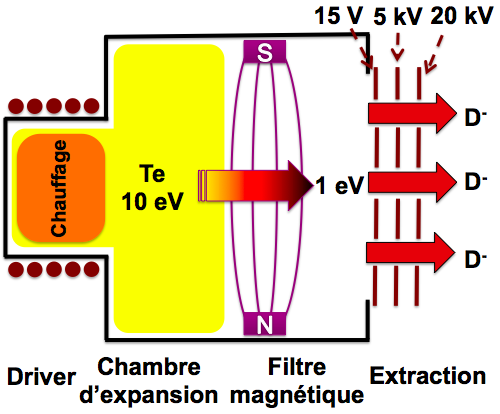
\includegraphics[width=1\textwidth]{figures/sourceIPP.png}
\captionsetup{justification=raggedright, singlelinecheck=false}
\captionof{figure}{Schéma de principe de l'un des "driver" de la source d'ions
négatifs de l'IPP Garching.}\label{IPPIonSource}
\end{minipage}\qquad\qquad
\begin{minipage}{0.40\textwidth}
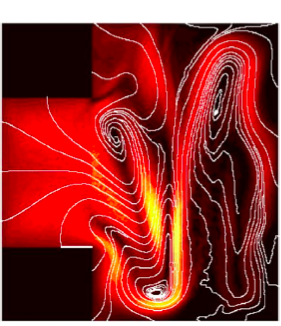
\includegraphics[width=0.9\textwidth]{figures/sourceIPPcourant.png}
\captionsetup{justification=raggedright, singlelinecheck=false}
\captionof{figure}{Dérive du flux électronique
le long de la barrière de champ magnétique.}\label{IPPIonSourcecourant}
\end{minipage}
\end{minipage}
\vspace{5 mm}

Depuis quelques années, le développement de la source fait notamment 
face à un problème majeur vis-à-vis de la non-uniformité du courant extrait, bien plus
important dans la partie haute de la source que dans sa partie basse (voir sur la
figure~\ref{IPPIonSourcecourant}). 
Pour comprendre l'origine de ce phénomène et corriger l'inhomogénéité du plasma,
de sérieux efforts ont été entrepris, aussi bien au niveau de la modélisation que
de l'expérimentation. 

L'une des pistes expérimentales étudiées change totalement de concept : au
lieu d'utiliser le champ magnétique pour filtrer les électrons énergétiques
l'idée est plutôt de s'en servir pour les confiner au centre d'une colonne de
plasma en rotation autour d'un axe magnétique (voir le schéma de la
figure~\ref{CYBELEIonSource}). Ce concept, en cours de développement au CEA de Cadarache avec la source Cybele, permettrait
d'obtenir une densité de plasma homogène sur toute la hauteur de la source. Dans
le cadre de la ligne IDN Siphore, de rapport d'aspect laminaire, ce type de
source s'adapte parfaitement à l'accélérateur Singap (pour Single Aperture
Photo-neutralization) qui neutralise le faisceau d'ions négatifs par
photo-détachement à l'aide d'un laser de 1 kW et d'une cavité de
Fabry-Perot~\parencite{SimoninHDR}.

Cybele en est toujours au stade expérimental, et un
code pouvant modéliser son fonctionnement pourrait grandement aider à son
développement, notamment pour simuler son intégration dans la ligne Siphore.

\begin{figure}[htbp]
\centering
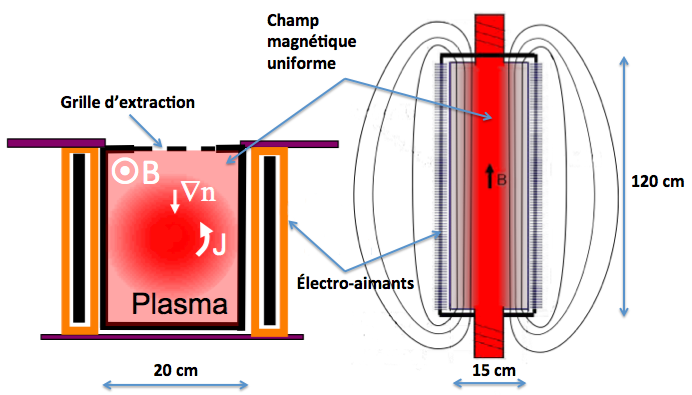
\includegraphics[width=0.7\textwidth]{figures/sourceSimonin1.png}
{\caption{Schémas de principe (vue de dessus à gauche et vue de face à droite)
de la source d'ions négatifs Cybele.}\label{CYBELEIonSource}}
\end{figure}


\section*{État de l'art}
Le comportement d'un plasma en présence d'un champ magnétique a été
longuement étudié et se trouve maintenant décrit dans de nombreux ouvrages sur
la physique des plasmas.
Les premières expérimentations dans les années 1950-1960 sur le confinement
magnétique du plasma démontrèrent l'existence d'un régime de transport classique
de type diffusif suivant une loi d'échelle en 1/B$^2$, puis, à plus haut champ
magnétique, l'apparition d'un régime de transport anormal variant plutôt en
1/B~\parencite{Bohm,Simon55,Yoshikawa,Janes,Rozhansky}. Les travaux plus
récents sur ce sujet montrent une nette distinction de
comportement entre les plasmas chauds de fusion et les plasmas froids, comme
discuté maintenant.

Pour les plasmas chauds, la littérature est actuellement dédiée en majeure
partie à l'étude du transport turbulent et de la grande variété d'instabilités qui
se développent et dégradent le confinement magnétique. De nombreuses
publications donnent des preuves expérimentales et une caractérisation de ces
phénomènes. Les théories et modèles correspondants sont typiquement basés sur
les approximations suivantes :

\begin{itemize}
  \item l'ionisation (quasiment) totale du plasma ;
  \item une agitation thermique importante des particules ;
  \item la forte magnétisation des électrons et des ions par un champ de
  plusieurs Teslas confinant le plasma dans un volume fini ;
  \item l'interaction de type Spitzer (collisions coulombiennes) entre les
  particules.
\end{itemize}

Dans les méthodes standards de modélisation, on retrouve les théories fluides de
la Magnéto-hydrodynamique
 (MHD) introduite
par Alfvén~\parencite{Alfven} et des vitesses de dérive~\parencite{SarazinPhD}
ou encore celle du centre-guide pour les modèles
particulaires~\parencite{Taylor,Lee,Garbet10}.
\footnote{La
théorie du centre-guide décompose le mouvement des particules en un mouvement
circulaire rapide superposé au déplacement d'un centre-guide parallèlement et
perpendiculairement au champ magnétique. La MHD, généralisation de la mécanique
des fluides, assimile le plasma à un fluide unique dans lequel l'inertie est
essentiellement due aux ions et la mobilité reliée aux
électrons~\parencite{Rax} ; elle est utilisée principalement pour suivre
la dynamique rapide d'un plasma, les phénomènes d'ondes, obtenir l'équilibre et
 étudier les macro-instabilités (modes "kink" et "sausage").
L'approche fluide des vitesses de dérive est quant à elle préférée pour étudier
l'évolution lente de l'équilibre et les micro-instabilités responsables du
transport turbulent : c'est l'approche que nous étudions dans cette thèse pour décrire les plasmas de bord des tokamaks.}

Dans le domaine des plasmas froids, une autre méthodologie s'est développée du
fait des conditions de plasmas et des intérêts de recherche
différents. En effet, les sources plasmas magnétisées qui nous intéressent
se distinguent des plasmas de fusion sous plusieurs aspects :

\begin{itemize}
  \item du fait de la faible intensité du champ magnétique (de l'ordre de
  0.01~T), seuls les électrons sont magnétisés, le rayon de Larmor ionique
  dépassant souvent la taille caractéristique du système ;
  \item la matière n'est que partiellement ionisée, l'interaction avec
  le gaz neutre influençant de façon prédominante le transport dans le plasma ;
  \item le plasma n'est pas confiné sur des lignes de champ fermées et
  l'interaction avec les parois est omniprésente, celles-ci agissant comme de
  parfaits puits de particules et d'énergie pour le plasma\footnote{
  En l'absence de confinement, le temps de résidence d'une particule dans le
  système est considérablement diminué et les distributions en vitesses des
  espèces peuvent s'écarter de façon notable de distributions maxwelliennes.}.
\end{itemize}

Le transport dans ces sources se décrit habituellement par des modèles fluides
de type Dérive-Diffusion~\parencite{Porteous,Lieberman,Rozhansky} quand les
plasmas sont suffisamment collisionnels. Des modèles
cinétiques Particles-In-Cell (PIC) avec des opérateurs collisionnels
Monte-Carlo~\parencite{PIC3D,Adam} ou hybrides
fluide-cinétique~\parencite{BoeufGarrigues} peuvent aussi être utilisés quand
une connaissance détaillée de la fonction de distribution devient nécessaire
(interactions ondes-particules, population à plusieurs niveaux d'énergie), mais
ils requièrent des ressources et des temps de calculs bien plus conséquents que
leurs homologues fluides, ce qui les rend bien moins adaptés aux études
paramétriques. De plus, la plupart de ces travaux de modélisation se focalisent
sur la performance et la caractérisation des décharges pour des applications
spécifiques (\parencite{Lieberman} et références inclues) et, excepté quelques
récentes études analytiques de colonnes de plasma idéales
(stationnaires~\parencite{Sternberg}, infinie suivant la direction axiale et de
symétrie axiale~\parencite{Fruchtman09}), très peu de travaux sont dédiés à la
compréhension du transport magnétisé en soi.

\begin{center}
\rule{0.5\textwidth}{1pt}
\end{center}


La connaissance sur le transport magnétisé dans les plasmas froids magnétisés
peut se résumer ainsi :

\textbf{1}. Le champ magnétique piège les électrons dans des orbites
cyclotroniques, ce qui rend leur transport fortement anisotropique. Selon
l'approche fluide standard~\parencite{Chen,Rozhansky,Lieberman,Rax}, les
coefficients de transport magnétisés prennent la forme de
tenseurs.
Considérons le flux électronique $\mathbf G_e$ en l'absence de champ magnétique
:

\begin{equation}
\mathbf G_e = \mu_e n_e\mathbf E - D_e\nabla(n_e)
\end{equation}

avec $\mu_e$ et $D_e$ les coefficients de mobilité et de diffusion, $n_e$ la
densité électronique et $\mathbf E$ le champ électrique. Le flux
électronique $\boldsymbol{\Gamma}_e$ en présence d'un champ magnétique est alors
donné par :
\begin{equation}
\label{MagnetizedFlux}
\boldsymbol{\Gamma}_e = \frac{1}{1+h_e^2}(\mathbf G_e + (\mathbf
h_e\cdot\mathbf G_e)\mathbf h_e-\underbrace{\mathbf h_e\times\mathbf
G_e}_\text{dérive})\equiv n_e\boldsymbol{\mu}_e\cdot\mathbf
E-\mathbf{D}_e\cdot\nabla(n_e)
\end{equation}
\begin{equation}
\mathbf h_e=\mu_e\mathbf B=\frac{e}{m_e\nu_e}\mathbf
B=\frac{\omega_{ce}}{\nu_e}\mathbf b
\end{equation}
où $\mathbf B$ est le champ magnétique et $h_e=|\mathbf h_e|$ est le paramètre
de Hall mesurant l'influence du champ
magnétique sur le transport collisionnel. \eqref{MagnetizedFlux} donne la
définition d'un tenseur de mobilité $\boldsymbol{\mu}_e$ dont les composants
diagonaux sont très anisotropiques :
 
\begin{itemize}
  \item $\mu_{e\para}=\mu_e$ parallèlement à $\mathbf B$
  \item $\mu_{e\perp}$ perpendiculairement à $\mathbf B$ :
\end{itemize}

\begin{equation}
\mu_{e\perp}=\frac{1}{1+h_e^2}\mu_e\approx\frac{m_e\nu_e}{eB^2}
\end{equation}
Le tenseur de mobilité a aussi des composants non-diagonaux :

\begin{equation}
\mu_{e\times}=\frac{h_e}{1+h_e^2}\mu_e\approx\pm\frac{1}{B}
\end{equation}

Ils décrivent le flux d'électrons dans la direction $\mathbf
B\times\mathbf G_e$, composé de la dérive $\mathbf E$x$\mathbf B$ (partie
advective de $\mathbf G_e$) et de la dérive diamagnétique (partie diffusive de
$\mathbf G_e$). Quand la configuration étudiée est de symétrie cylindrique et
que le champ magnétique est dans le plan ($z$,$r$), cette dérive se referme sur elle-même dans la direction
azimutale et n'interfère pas directement avec le transport des particules vers
la paroi (voir figure~\ref{Contextederive}-a). En conséquence le transport est
contrôlé uniquement par $\mu_{e\para}$ et $\mu_{e\perp}$, avec un ratio $\mu_{e\para}/\mu_{e\perp}$ pouvant aller
jusqu'à 8 ordres de magnitude ; le confinement est alors dû à la très faible
valeur de $\mu_{e\perp}$.
\vspace{1cm}

\textbf{2}. Quand la mobilité dans la direction perpendiculaire au champ
magnétique est fortement réduite ($\mu_{e\para}\gg\mu_{e\perp}$) le plasma a tendance à
développer des instabilités et de la turbulence, ce qui amplifie
considérablement le transport transverse des électrons. Un grand nombre de
publications font état de ce transport "anormal" (i.e.
$\mu_{e\perp}$ plus grand que dans l'expression classique donnée précédemment)
lié à ces instabilités dans des sources plasmas froids
basse-pression~\parencite{Bradley,Adam}.

Des simulations PIC ont aussi montré
la présence d'un transport turbulent et de phénomènes instationnaires, par
exemple dans le cas des propulseurs à effets Hall~\cite{Adam08}. La
compréhension des phénomènes de transport anormaux dans les plasmas froids
basse-pression reste superficielle et on ne peut ni quantifier leur effets, ni
même donner de lois d'échelle utilisables.
Les théories développées dans le cadre de la recherche sur la fusion
thermonucléaire contrôlée ne semblent pas non plus pouvoir s'appliquer du fait de conditions et
de paramètres plasmas très différents. Par manque de connaissance,
beaucoup d'auteurs s'appuient sur la formule empirique proposée par Bohm
$\mu_\perp=1/16B$~\parencite{Bohm} sans plus de justifications.
\vspace{1cm}

\begin{figure}[htbp]
\centering
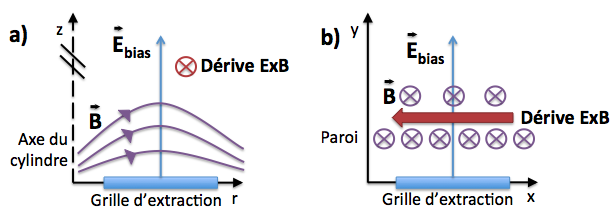
\includegraphics[width=\textwidth]{figures/derives.png}
{\caption{Configurations "Filtre magnétique" pour
\textbf{a)} une dérive azimutale et \textbf{b)} une dérive
bloquée. Dans le deuxième cas, le plasma développe une
asymétrie (effet Hall) et fait passer le flux
électronique au travers du filtre au niveau de la
paroi.}\label{Contextederive}}
\end{figure}

\textbf{3}. Avec la présence de parois conductrices, le transport dans les
plasmas froids est généralement non-ambipolaire, i.e. les flux ioniques et
électroniques ne sont localement pas égaux et les courants se rebouclent à
travers les murs~\parencite{Rozhansky}, provoquant un effet de "court-circuit".
Dans de nombreuses configurations, les électrons ont ainsi tendance à quitter
le plasma le long des lignes de champ tandis que les ions sont perdus sur toute
la surface des parois, ce qui rend les pertes globales bien plus importantes
que celles prédites par la théorie ambipolaire.

Cet effet, découvert par Simon en 1955~\parencite{Simon55}, peut dans certains
cas expliquer le transport "anormal" observé mais reste encore souvent négligé,
comme l'a si bien illustré la polémique récente dans la littérature
(e.g.~\parencite{Fruchtman,Simon08,Fruchtman08}). De plus, bien que la relation
de Boltzmann,
\begin{equation}
q_e\mathbf
E =\frac{\nabla (n_e T_e)}{n_e}
\end{equation}
ne soit pas justifiée dans la direction perpendiculaire au champ magnétique,
plusieurs récentes publications font l'hypothèse irréaliste d'un transport
totalement ambipolaire~\parencite{Fruchtman,Nasi}.
\vspace{1cm}

\textbf{4}. Dans les géométries cylindriques, la dérive due au champ magnétique
est dans la direction azimutale et n'interfère pas directement avec le
confinement du plasma, mais dans les
configurations où cette symétrie est absente, la dérive magnétique est bloquée
par la paroi et elle joue un rôle majeur dans le transport perpendiculaire
(figure~\ref{Contextederive}-b). La dérive bloquée a alors tendance à déformer
le plasma, de façon similaire à la polarisation d'un solide par l'effet Hall.

Dans la configuration filtre, où la dérive ne se referme pas sur elle-même, on
peut donc s'attendre à ce que le transport transverse soit plutôt dominé par $\mu_{e\times}$ et suive une loi d'échelle en $1/B$, tout comme le transport
turbulent. Cet effet est critique pour la source d'ITER car il
entraîne la non-uniformité du courant d'ions négatifs extraits, comme le montre
les mesures expérimentales sur la source de l'IPP Garching.

 \section*{Contexte local} Le
groupe GREPHE du LAPLACE a une grande expérience dans la modélisation des plasmas froids magnétisés. Depuis le milieu des années 90, où il a commencé à s'impliquer dans la modélisation des propulseurs à effet Hall (GDR propulsion Plasma, ANR TELIOPEH, contrats SNECMA, SNES, ESA), le groupe a graduellement
étendu son domaine de recherche à d'autres sources de plasma magnétisé
(PLASMODIE, ESSILOR). En 2006, le groupe GREPHE
a été choisi pour concevoir un modèle numérique auto-consistant de la source de
Garching\footnote{Ce modèle, MAGMA, décrit l'ensemble des aspects
physiques de la source d'une manière auto-consistente (chauffage RF, cinétique,
déplétion du gaz neutre, chimie de l'hydrogène et processus de surface). Dans
son état actuel d'avancement, le développement de MAGMA rencontre de sérieuses
difficultés pour modéliser le transport au niveau du filtre magnétique, ne
pouvant obtenir de solution stable et convergée qu'en dessous d'une certaine
intensité de champ magnétique.} dans le cadre de plusieurs contrats avec le CEA/EURATOM de
Cadarache, la Fédération de Recherche sur la Fusion Magnétique, ITER et le
projet ANR ITER-NIS (2008--2011). Certains des membres du GREPHE sont de plus
impliqués dans le projet ANR Blanc EPIC (LPP Polytechnique 2011) sur le nouveau
concept de propulseur ion-ion PEGASES, qui utilise lui aussi un
champ magnétique en configuration filtre. 

Depuis 2012, le groupe GREPHE est responsable du projet ANR METRIS, dont
l'objectif général est d'améliorer la compréhension du transport magnétisé dans
les plasmas froids en l'étudiant comme sujet à part entière. Le projet
contient deux volets principaux :

\begin{itemize}
  \item l'élaboration d'une expérimentation dédiée à l'étude du transport
magnétisé~\parencite{Baude} ;
\item le développement d'un modèle fluide robuste, qui est
le sujet de cette thèse.
\end{itemize}
 
 La première année de
 le thèse s'est déroulée au sein de l'équipe théorique GP2B de l'Institut de
 Recherche sur la Fusion Magnétique du CEA de Cadarache, avec laquelle le GREPHE
 a entamé une collaboration dans le contexte de ce projet. Elle a consisté à
 étudier les méthodes utilisées dans la recherche
 sur la fusion pour modéliser le transport fortement magnétisé afin de les
 appliquer au domaine des plasmas froids. La suite de la thèse s'est passée à
 Toulouse au GREPHE et a été dédiée au développement d'un nouveau modèle,
 combinant les techniques spécifiques aux deux communautés.
 
\section*{Organisation de la thèse}
	Le premier chapitre de cette thèse rappelle une partie des concepts 
	fondamentaux de la physique des plasmas, nécessaires à la fois à la bonne
	compréhension du transport magnétisé et à l'auto-suffisance du manuscrit. Nous
	y parlons des plasmas, des phénomènes de transport et des échelles
	caractéristiques que nous serons amenés à rencontrer tout au long du manuscrit.
	La fin du chapitre concerne la théorie fluide qui est utilisée dans les deux
	modèles de transport magnétisé que nous étudions.
	
	Le chapitre II compare deux approches de modélisation à travers une
	discussion sur les approximations de l'équation de conservation de la quantité
	de mouvement : l'équation de Dérive-Diffusion et son homologue magnétisée,
	largement utilisées dans la communauté des plasmas froids, sont basées sur des
	hypothèses de stationnarité et de forte collisionnalité du plasma. L'approche
	des vitesses de dérive suppose quant à elle une forte magnétisation de
	l'ensemble des particules.
	
	Le troisième chapitre est consacré au code TOKAM2D qui est utilisé depuis de
	nombreuses années dans l'équipe GP2B pour étudier le transport des particules
	dans le plasma de bord des tokamaks. Nous commençons par décrire son modèle,
	basé sur l'approche des vitesses de dérive, puis nous illustrons par des cas
	 simples les différentes modifications qui lui ont été apportées afin de
	 l'adapter aux sources magnétisées basse-pression.
	
	Dans le chapitre IV, nous présentons MAGNIS, le nouveau code développé dans le
	cadre de la thèse. C'est un modèle fluide, quasineutre, qui décrit le transport
	du plasma dans le plan perpendiculaire au champ magnétique. Les conditions aux
	limites sont dérivées d'une théorie classique de gaine (intégrant le critère
	de Bohm), et contiennent un maximum de considérations physiques. Nous
	détaillons dans une deuxième partie le schéma numérique élaboré spécialement pour le modèle.
	
	 Le dernier chapitre porte sur l'étude de trois cas de test simplifiés,
inspirés d'expérimentations réelles. Chacun des cas possède sa problématique
spécifique, et est représentatif d'une géométrie magnétique
particulière :
\begin{itemize}
  \item la configuration de filtre magnétique (ou barrière magnétique) pour le
  propulseur électrostatique PEGASES ou la source d'ions négatifs du système IDN d'ITER ;
		\item une colonne de plasma avec un champ uniforme, caractéristique de
		nombreuses expérimentations, dont la source d'ions Cybele ;
		\item une configuration typique de plasma de bord de tokamak, avec un champ
		magnétique intense et l'apparition d'un transport de nature turbulente.
\end{itemize}


%\bibliographystyle{apalike}
%\bibliography{biblio}
\end{refsection}
\renewcommand{\thefigure}{\thesection.\arabic{figure}}
\renewcommand{\theequation}{\thechapter-\thesection.\arabic{equation}}
%\adjustmtc[1]

